\section{ACSCH Inverse Hyperbolic Cosecant Function}

\subsection{Usage}

Computes the inverse hyperbolic cosecant of its argument.  The general
syntax for its use is
\begin{verbatim}
  y = acsch(x)
\end{verbatim}
where \verb|x| is an \verb|n|-dimensional array of numerical type.
\subsection{Function Internals}

The \verb|acsch| function is computed from the formula
\[
   \mathrm{csch}^{-1}(x) = \sinh^{-1}\left(\frac{1}{x}\right)
\]
\subsection{Examples}

Here is a simple plot of the inverse hyperbolic cosecant function
\begin{verbatim}
--> x1 = -20:.01:-1;
--> x2 = 1:.01:20;
--> plot(x1,acsch(x1),x2,acsch(x2)); grid('on');
\end{verbatim}


\centerline{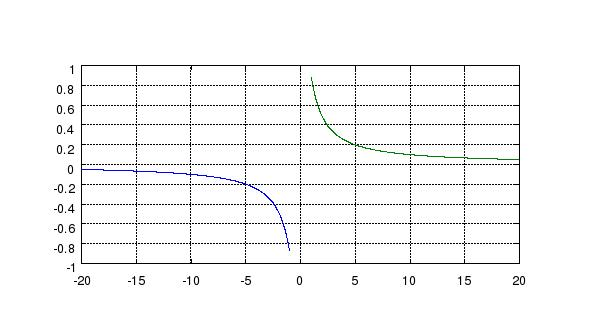
\includegraphics[width=8cm]{acschplot}}

